\chapter{Fit to the reference channel \LbToLcmunu}
\label{sec:Normalisationfit}
This chapter describes the measurement of the signal yield \NLc in the normalisation channel \LbToLcmunu (\LcTopKpi). 
The method is different to the one in the signal channel \LbToDpmunuX due to several reasons:
All of the final state particles of the subdecay \LcTopKpi can be reconstructed and the statistics is much higher. 
Going through an intermediate resonance it is possible to see a clear \Lc mass peak as shown in Figure \ref{fig:plot_Lc_M}.
In \LbToDpmunuX the major part of the decays was non-resonant.
The small sidebands indicate a small combinatorial background in the subdecay \LcTopKpi.
The background contribution coming from a random combination of a \Lc with a muon can be estimated by investigating the wrong sign final states combinations \Lc\mup.
Since a \Lb cannor decay into a \Lc\mup due to charge conservation, this unphysical combination serves as model for randomly combined \Lc\mun.
The second reason why a different method is chosen compared to the \LbToDpmunuX channel is the fact that the \Lb can decay in several excited \Lc states, in the following denoted as \Lcstar for any excited \Lc state.
Contrary to \LbToDpmunuX, the yield of the decay \LbToLcmunu is measured exclusively.
This means that all decays going through intermediate resonances etc. have to be subtracted.
It has been shown in \cite{SL_Vub}, that the \LbToLcmunu data is polluted by the decays \decay{\Lb}{\LcRes{(2595)}\mun\neumb} and \decay{\Lb}{\LcRes{(2625)}\mun\neumb}.
These excited \Lcstar baryons instantly decay for instance in \Lc\pip\pim or \Lc\piz. 
If these (neutral) pions are not reconstructed, this decay cannot be distinguished from \LbToLcmunu by its topology.
Thus, a fit of \logIP, a measure vor the vertex quality, as done in Chapter \ref{sec:Signalfit} would not help to distinguish between \LbToLcmunu and \decay{\Lb}{\Lcstar\mun\neumb} and a different approach for the determination of \NLc has to be chosen.

The solution of the latter problem is to fit the corrected \pKpi\mun alias \Lb mass.
It has been stated in chapter \ref{sec:Selection}, that the corrected \pKpi\mun or \Lb mass peak close to the nominal \Lb mass, if the missing particle is massless.
Concerning the \decay{\Lb}{\Lcstar\mun\neumb} decays, on misses not only the neutrino, but furthermore massive particles like the neutral pions.
Thus, the corrected \Lb mass is shifted to lower mass, enabling a fit to distinguish between the semileptonic \Lb decay into a \Lc or \Lcstar.
This assumption on the corrected mass is verified in section \ref{sec:FitCorrectedMass}.
\begin{figure}[ptb]
    \centering
	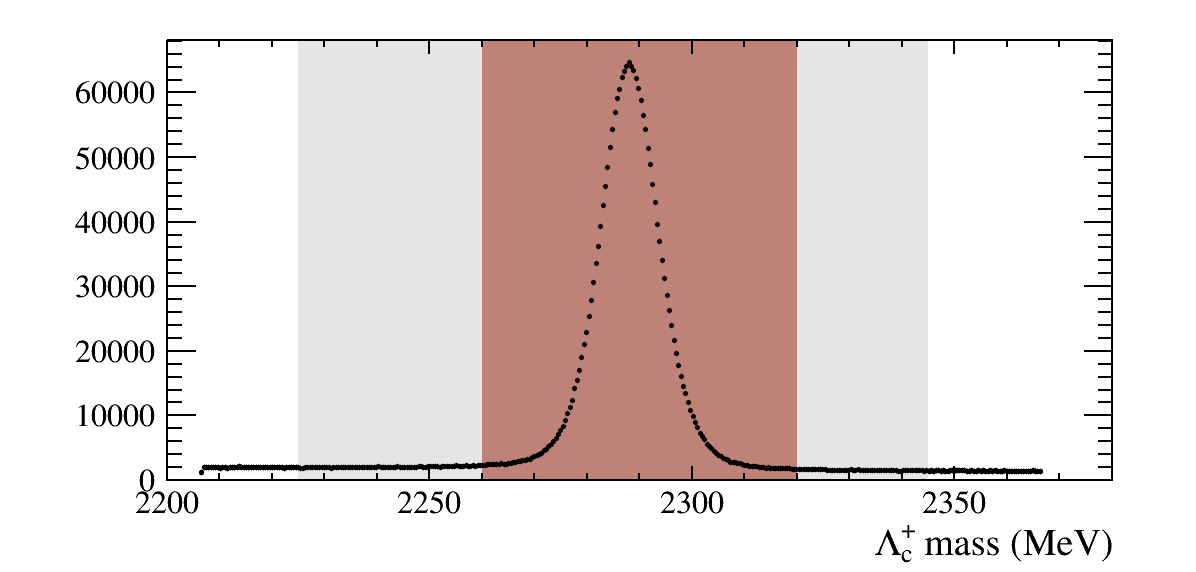
\includegraphics[width=\textwidth]{LbToLc/fancyplots/Lc_M_bands}	
	\caption{Plot of the invariant \pKpi mass distribution. A clear mass peak identified as the \Lc can be seen. The dark shaded area indicates the chosen signal band and the light grey area the background bands for the sideband subtraction.}
	\label{fig:plot_Lc_M_bands}
\end{figure}

\section{Reduction and handling of backgrounds}
This section describes the ways how different sources of backgrounds are either handled or reduced.

\subsection{Non \Lc background}
As already mentioned the reconstruction of \pKpi yields a nice mass peak forming the hadronically decaying \Lc, which can be seen in figure \ref{fig:plot_Lc_M}. 
Events outside of this peak can be explained by a random combination of a proton, a kaon and a pion.
Nonetheless there is also a certain amount of this ``combinatorial" background in the peak region.
It is statistically eliminated by a sideband subtraction (see section \ref{sec:Sidebandsubtraction}).
The signal band is chosen to lie in the invariant \pKpi mass range between $\in \left[2260, 2320\right]\mev$.
The background bands are M(\pKpi) $\in \left[2225, 2260\right]\mev$ or M(\pKpi) $\in \left[2320, 2345\right]\mev$.
The chosen bands are visualised in Figure \ref{fig:plot_Lc_M_bands}.

\subsection{Random combinations of \Lc and \mun}
The next possible source of backgrounds are random combinations of a correctly reconstructed \Lc baryon and a muon \mun. 
Due to the missing neutrino \neumb there is no signal mass peak and it is not possible to use a sidebandsubtraction on the invariant \pKpi\mun (\Lc\mun) mass.
Thus, wrong sign events, i.e. ``unphysical" events with a \Lc\mup in the final state as explained above are used to estimate the amount of random \Lc\mun background.
It is assumed that the shape and the number of the wrong sign events are compatible with the shape and number of random \Lc\mun combinations.
Finally, the amount of wrong sign events is subtracted from the ``right sign" events to statistically eliminate this source of backgrounds.

\subsection{Peaking backgrounds}
The third source of backgrounds is peaking background from partially reconstructed decays.
This means, that there are physical decays mimicking to be signal since some of the particles are not reconstructed.
In this case the \LbToLcmunu data is polluted by the decays \decay{\Lb}{\LcstarRes{(2595)}\mun\neumb} and \decay{\Lb}{\LcstarRes{(2625)}\mun\neumb} \cite{SL_Vub}.
A \Lcstar subsequently decays into a \Lc and not reconstructed neutral remnant, e.g. \piz, \pip\pim.
Since this decay happens instantaneously it looks the same as \LcTopKpi in the detector.
As already explained, those decays can be distinguished from \LbToLcmunu by their corrected \Lb mass.
Thus, these kind of backgrounds are not subtracted from the data, but rather included as component into the fit to the corrected \Lb mass.

\section{Fit to the corrected \pKpi\mun (\Lb) mass}
\label{sec:FitCorrectedMass}
In this chapter it is verified in a simulation, that the corrected \pKpi\mun mass is different for \LbToLcmunu, \decay{\Lb}{\LcstarRes{(2595)}\mun\neumb} and \decay{\Lb}{\LcstarRes{(2625)}\mun\neumb}.
Figure \ref{fig:correctedMass_normalisation} shows the simulated corrected \pKpi\mun mass distributions for the different decays.
\begin{figure}[hptb]
	\centering
	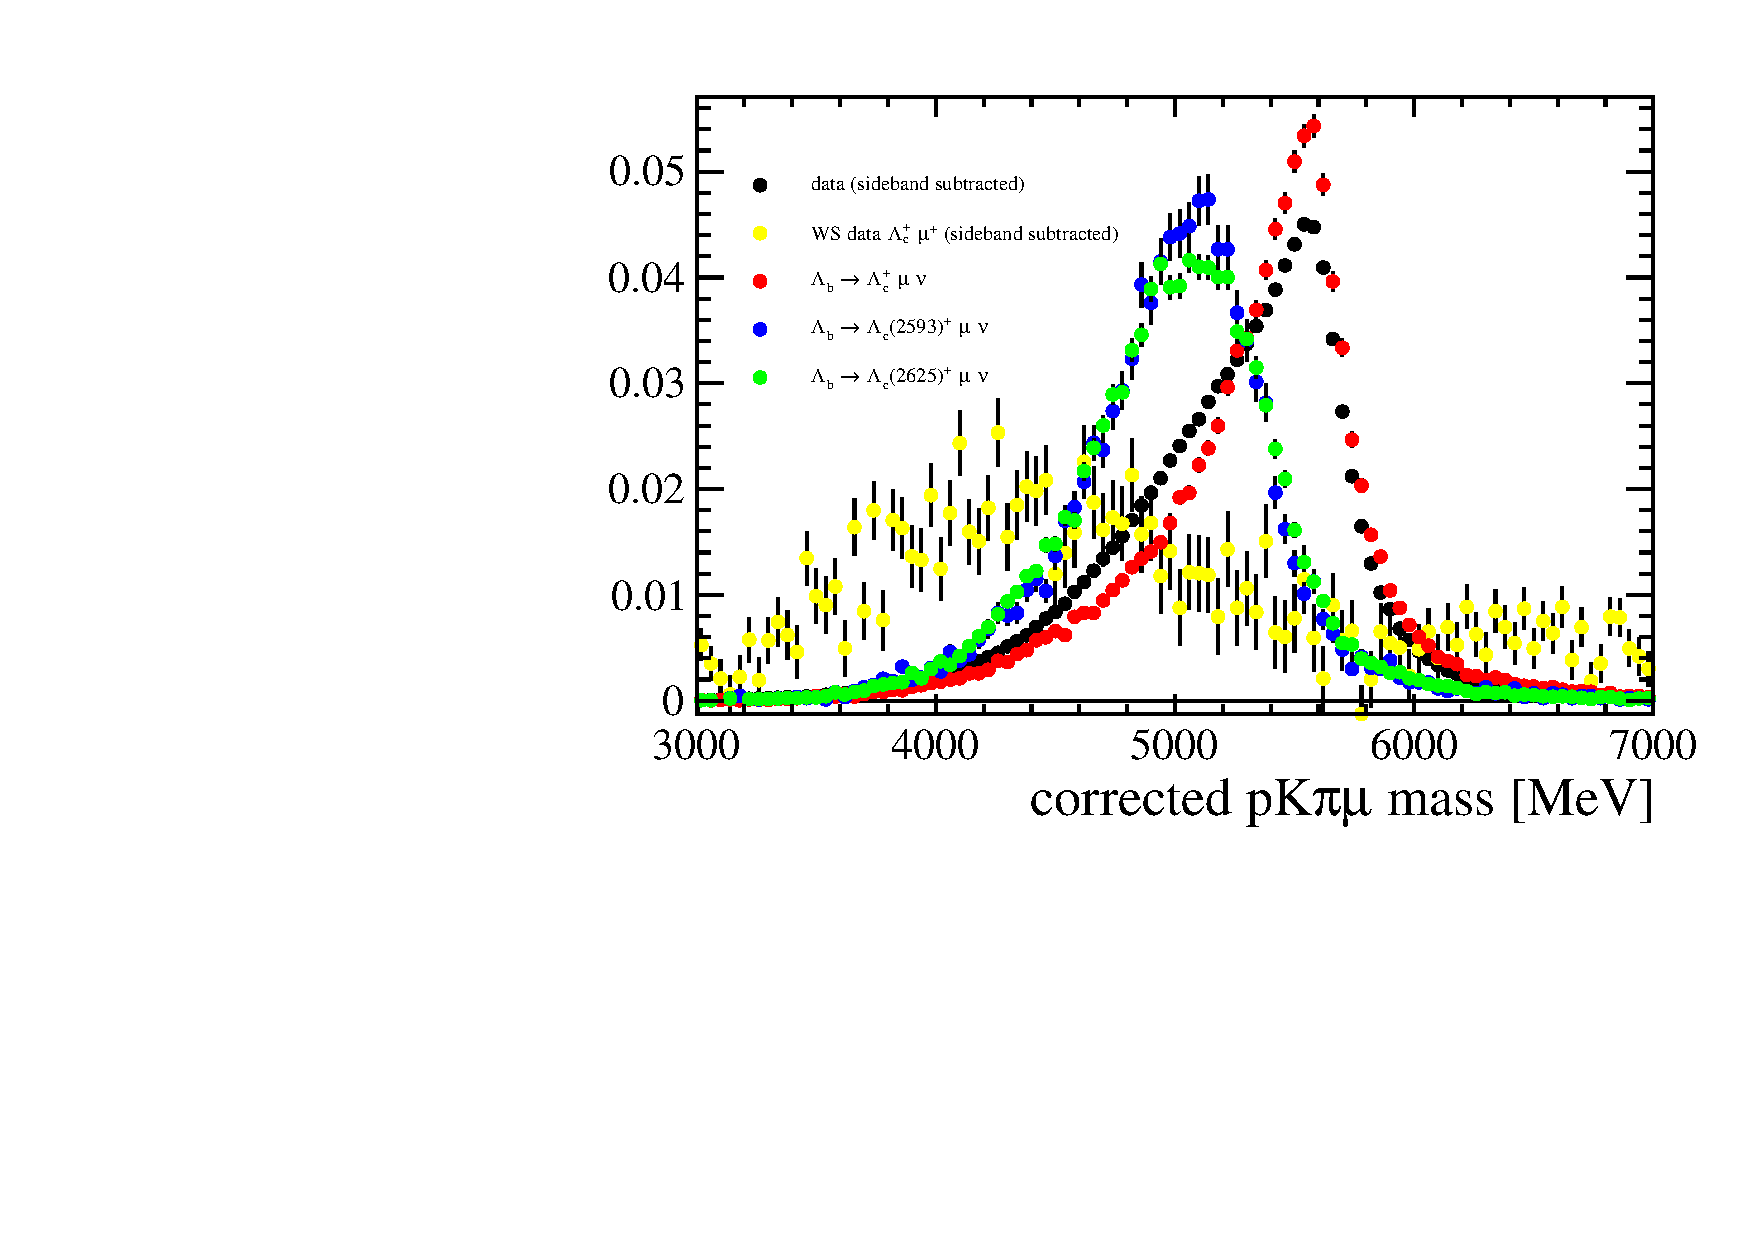
\includegraphics[width=0.75\textwidth]{LbToLc/correctedMass/correctedMass}
	\caption{Comparison of the \pKpi\mun corrected mass for the semileptonic \Lb decays via \Lc, \LcstarRes{(2595)} and \LcstarRes{(2625)} gained from simulation. The black points show the sideband subtracted data distribution. The shape of the combinatorial \Lc\mun background (WS events), which is
    subtracted for the fit, is shown in orange.}
	\label{fig:correctedMass_normalisation}
\end{figure}

With the help of Figure \ref{fig:correctedMass_normalisation}, one can draw the following conclusions:
\begin{itemize}
    \item The corrected \pKpi\mun mass indeed looks different for \LbToLcmunu and \decay{\Lb}{\Lcstar\mun\neumb} decays.
          It peaks around the nomimal \Lb mass for \LbToLcmunu whereas it is shifted to lower masses for the decays into the excited \Lcstar states. 
    \item It is not possible to distinguish in the \Lb corrected mass spectrum between the semileptonic \Lb decays into \LcstarRes{(2595)} and \LcstarRes{(2625)} as their shapes are too similar.
\end{itemize}
The latter conclusion is not really a problem since the only result of interest is the \LbToLcmunu signal yield. 
A distinction among the excited states is not needed.
In the fit there will be just one common component for both final states.
Having this in mind, the fit procedure is performed as follows:
\begin{enumerate}
    \item The data is sideband-subtracted using the \pKpi (i.e. \Lc) mass bands.
    \item The corrected \pKpi\mun mass distribution from wrong sing events is subtracted from the respective distribution from the right sign data.
    \item A fit of the \pKpi\mun mass is performed using the Beeston-Barlow method (see sec. \ref{sec:BeestonBarlow}) to account for uncertainties in the corrected mass templates from simulation. The fitted parameters are the \Lc signal yield and one common yield for the two excited \Lcstar channels.
\end{enumerate}
The results can be seen in figure \ref{fig:correctedMass_fit} and table \ref{tab:fit_correctedMass}. 
They are presented in different ways:
The left-hand side shows the fit result with the adjusted templates according to the Beeston-Barlow method, i.e. the templates have been modified binwise within their uncertainties to better match the data.
The agreement with the data is remarkable, even on a logarithmic scale, shown in the bottom row of Figure \ref{fig:correctedMass_fit}.
The right-hand side compares data and fitresult with the bare templates.
Slight deviations can be figured out here, above all in the tails with few statistics.
The \LbToLcmunu signal yield \NLc obtained by the fit to the corrected \pKpi\mun mass and required for the determination of \R is:
\begin{align*}
    \NLc = (\NLcvalscient \pm \NLcerrscient)\cdot 10^{\NLcexpscient}
\end{align*}
\begin{figure}[hptb]
	\centering
	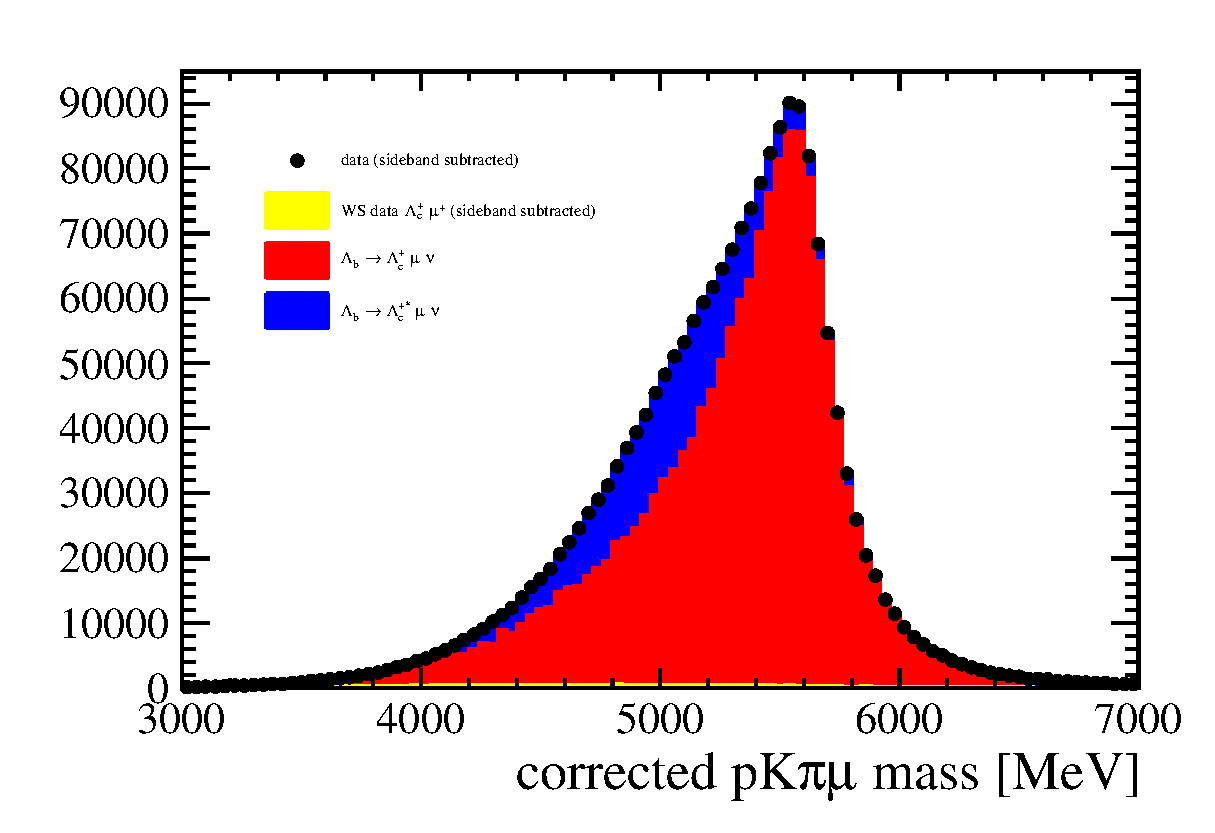
\includegraphics[width=0.49\textwidth]{LbToLc/correctedMass/fit_correctedMass}
	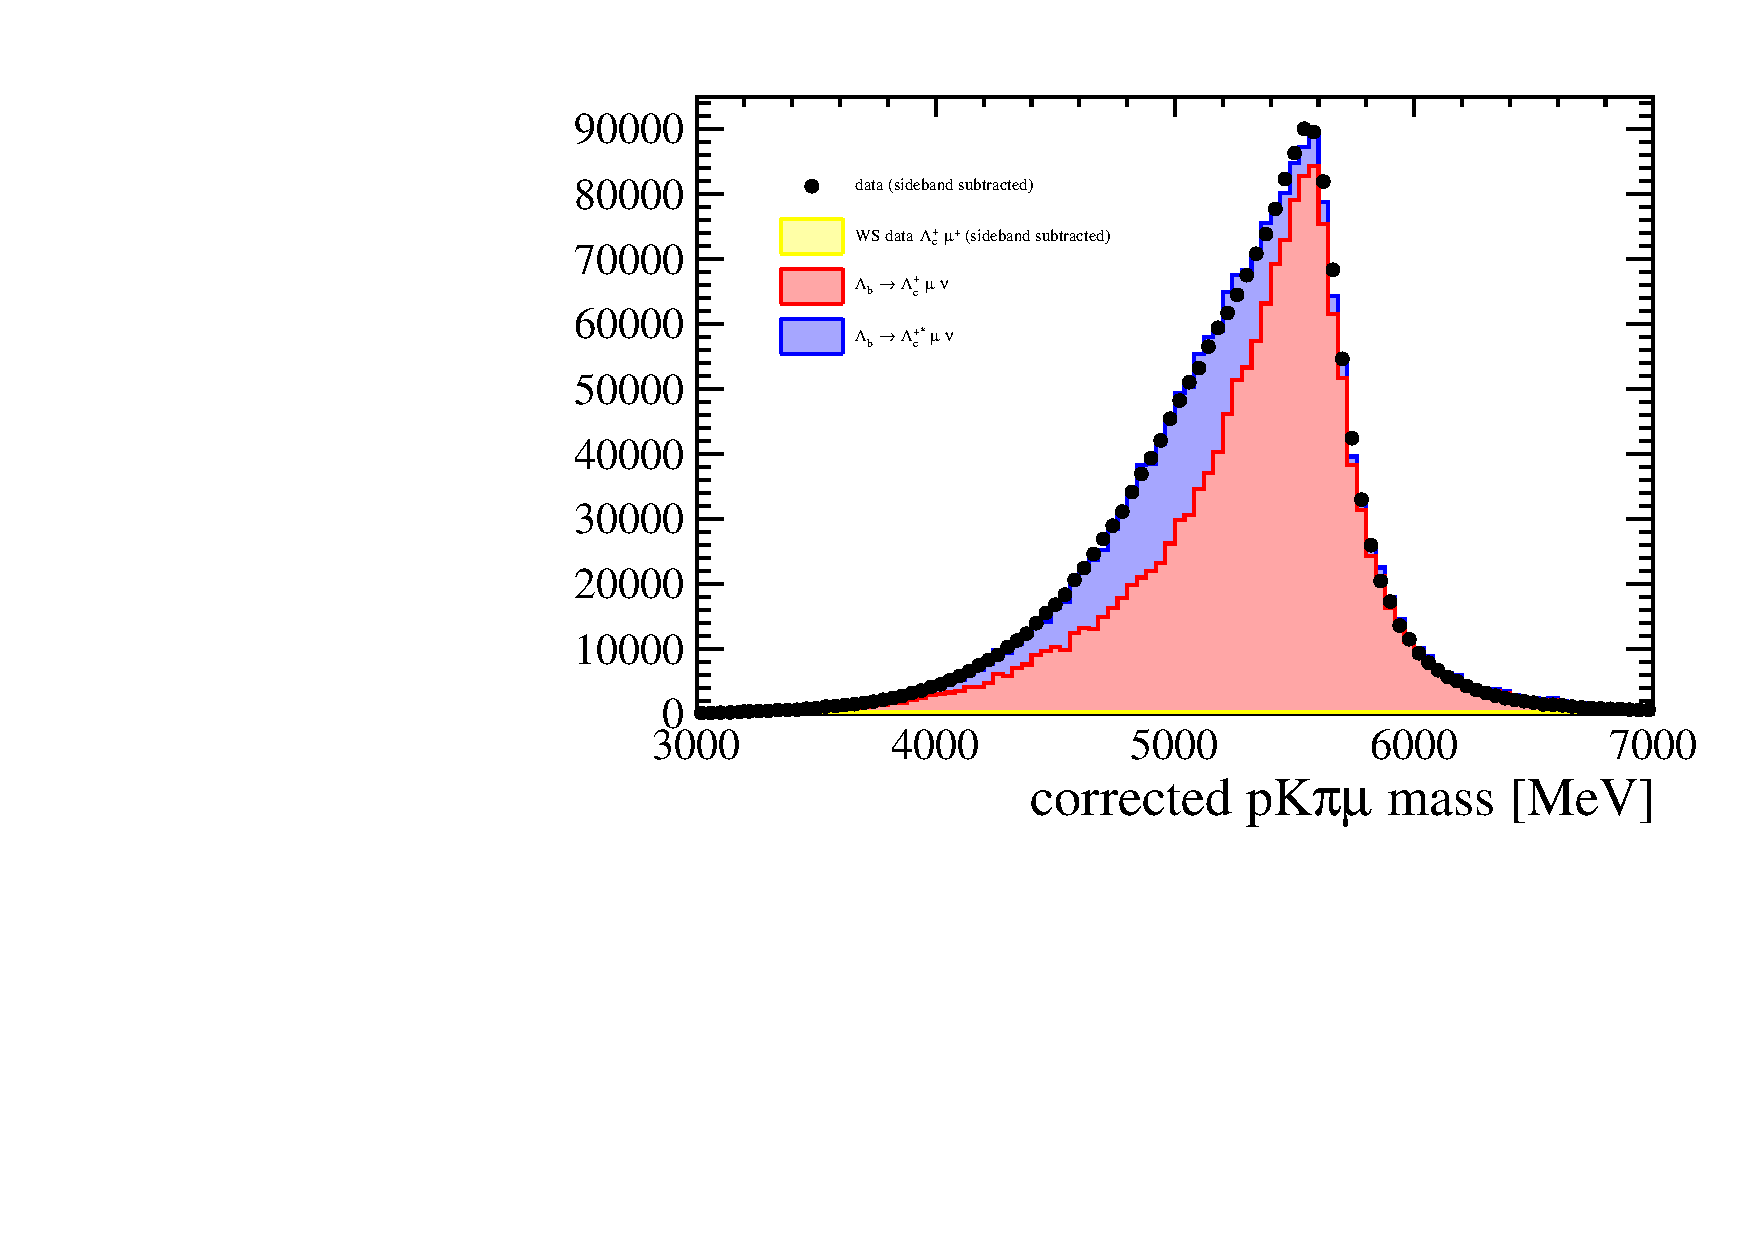
\includegraphics[width=0.49\textwidth]{LbToLc/correctedMass/fit_correctedMass_noBB} \\
	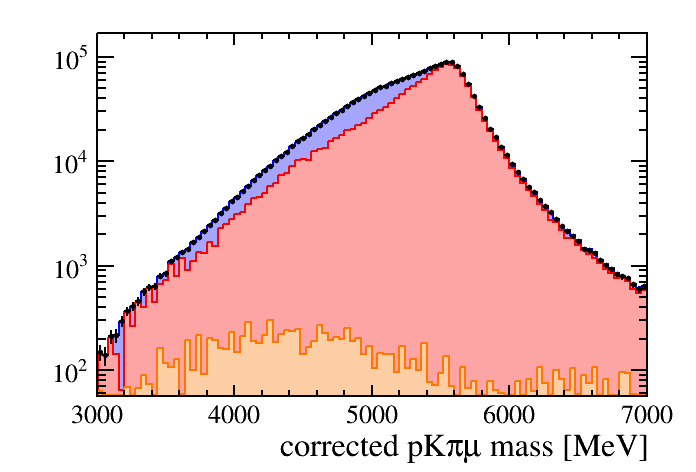
\includegraphics[width=0.49\textwidth]{LbToLc/correctedMass/fit_correctedMass_logscale}
	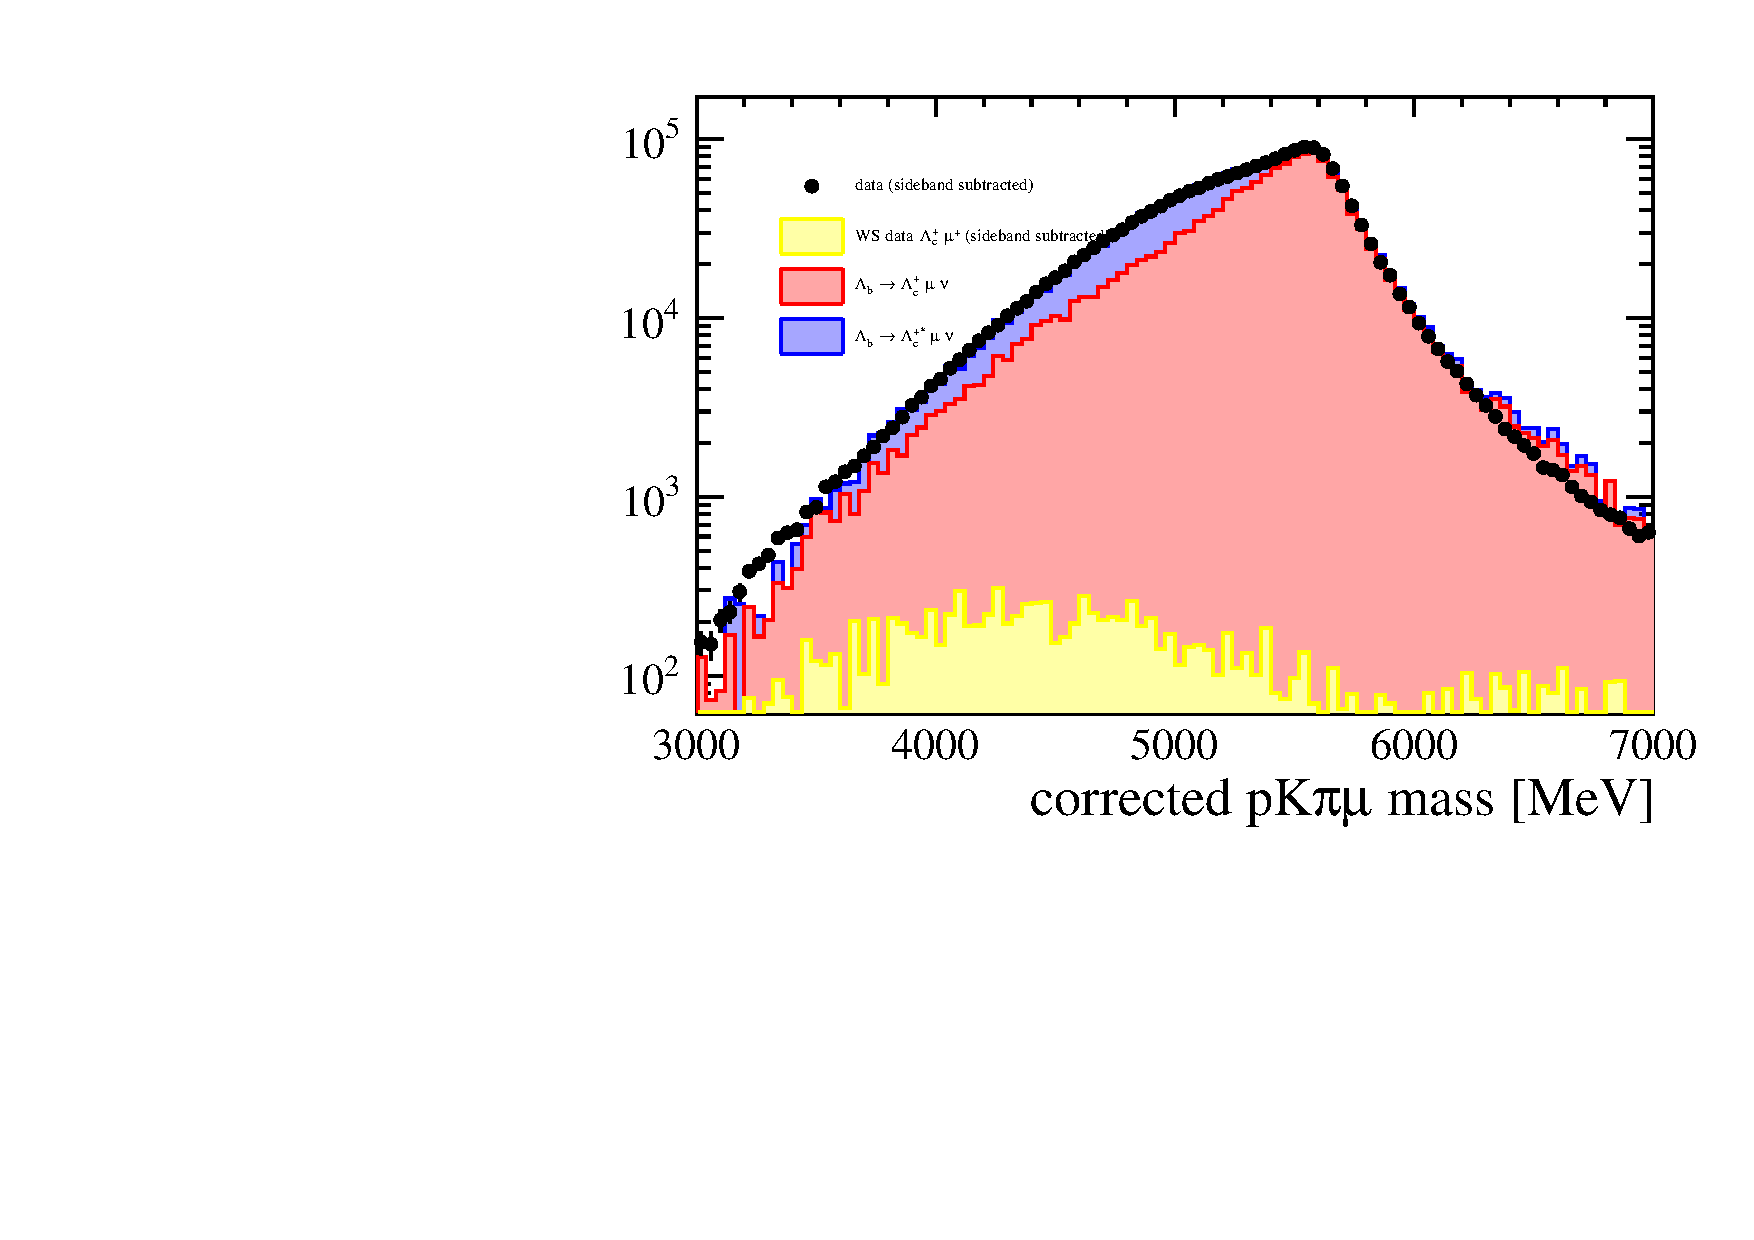
\includegraphics[width=0.49\textwidth]{LbToLc/correctedMass/fit_correctedMass_noBB_logscale}
	\caption{Fit to the \pKpi\mun corrected mass for the determination of the \LbToLcmunu signal yield. The left plot shows the fit result with the adjusted templates according to the Beeston-Barlow method, the right one the bare templates without any modification. The top row shows the result on a linear, the bottom row on logarithmic scale.}
	\label{fig:correctedMass_fit}
\end{figure}
 
\begin{table}[h]
    \centering
    \caption{Results of the \Lc corrected mass fit.}
    \label{tab:fit_correctedMass}
    $\begin{array}{lr@{\pm}l}
    \hline
    \text{Variable} & \multicolumn{2}{c}{\text{Value}} \\
    \hline
        \text{\Lc candidates \NLc}&(1.544 & 0.011) \cdot 10^{6}\\
\text{excited \Lcstar candidates}&(4.375 & 0.096) \cdot 10^{5}\\
\text{combinatoric background}&(1.196 & 0.033) \cdot 10^{4}\\

\hline
\end{array}$
\end{table}
    
